\begin{figure}[H]
	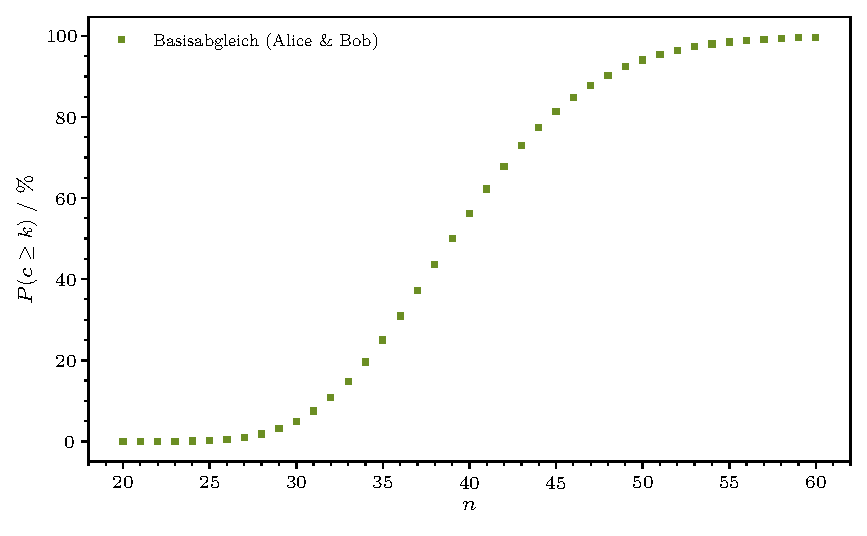
\includegraphics{build/kumuliert.pdf}
	\vspace{-1.5\baselineskip}
	\captionsetup{width=0.93\textwidth}
	\caption{Kumulierte Verteilung für das Auftreten von mindestens $k = 20$ passenden Basispaaren mit $p = \qty{50}{\percent}$
			 in $n$ Messungen zur Schlüsselgeneration.}
	\label{fig:kumuliert}
	\vspace{-2.5\baselineskip}
\end{figure}

\section{Auswertung}

Als Serie gleichartiger und unabhängiger Events lassen sich die Wahrscheinlichkeiten für das Eintreten der verschiedenen
Fälle in diesem Versuch mithilfe der Binomialverteilung
\begin{equation*}
	P(c = k) = f(k, n, p) = \pfrac{n!}{k!(n - k)!} \, p^k (1 - p)^{n - k}
\end{equation*}
bestimmen. Daraus folgt auch die in Abbildung \ref{fig:kumuliert} aufgetragene kumulierte Verteilung
\begin{equation*}
	P(c \geq k) = F(k, n, p) = \!\! \sum_{m \, = \, k}^n \! f(m, n, p)
\end{equation*}
für das Auftreten von $k$ oder mehr Ereignissen mit Einzelwahrscheinlichkeit $p$ aus den insgesamt $n$ diskreten Messungen.
Das zufällige Eintreten gleicher Basen hat $p = \qty{50}{\percent}$~und tritt bei den empfohlenen $n = 52$ Signalen in
$\qty{96.48}{\percent}$ der Fälle ausreichend oft für die geforderte Schlüssellänge $k = 20$ auf.



\subsection{Verschlüsselung einer Nachricht}

Wie zuvor beschrieben wird nun das Vorgehen zur Erzeugung eines zufälligen Schlüssels in Tabelle \ref{tab:schluessel}
implementiert. Zur Veranschaulichung sind gleiche Basiseinstellungen farblich hervorgehoben und die
Polarisationsdrehplattenpositionen von \glqq{Alice}\grqq{} angegeben.

\begin{longtable}[c]{rccrcc}
	\caption{Dokumentation des Signalaustauschs zur Erzeugung einer Verschlüsselung. Übereinstimmende Basen sind
			 \cbb{blau} hinterlegt. Zum besseren Verständnis sind zudem Winkeleinstellungen für die unterschiedlichen
			 Kombinationen von Basis und Bit eingetragen.}
	\label{tab:schluessel}
	\\
	\expandableinput{content/tabelle/schluessel.tex}
	\vspace{2.5\baselineskip}
\end{longtable}

Bei dieser Messreihe stimmen die Basen in 23 Fällen überein. Dieser Anzahl kann eine Wahrscheinlichkeit von
$\qty{7.84}{\percent}$ zugeordnet werden, was nach Vergleich mit Abbildung \ref{fig:verteilung} relativ nah am Maximum
der Verteilung und somit dem Erwartungswert liegt. Es folgt
\begin{equation*}
	\text{0 1 0 1 1 1 0 0 1 0 1 0 0 1 1 1 0 0 0 1 0 1 1}
\end{equation*}
als unabhängig von \glqq{Alice}\grqq{} und \glqq{Bob}\grqq{} bekannte Sequenz, deren erste 20 Stellen nun für den
Schlüssel festgelegt werden. Zur Kommunikation wird die \glqq{+}\grqq{} Basis gewählt.

\begin{table}[H]
	\centering
	\caption{Vorgehen von \glqq{Alice}\grqq{} zum Senden der Nachricht \texttt{TEST}.}
	\label{tab:alice}
	\begin{tabular}{lcccc}
		\expandableinput{content/tabelle/alice.tex}
	\end{tabular}
\end{table}

\begin{table}[H]
	\centering
	\caption{Vorgehen von \glqq{Bob}\grqq{} zum Empfangen der Nachricht \texttt{TEST}.}
	\label{tab:bob}
	\begin{tabular}{lcccc}
		\expandableinput{content/tabelle/bob.tex}
	\end{tabular}
\end{table}

Das Vorgehen zur Verschlüsselung durch Addition, zum Versenden der sicheren Nachricht, und dem abschließenden Entschlüsseln
sind in Tabelle \ref{tab:alice} für \glqq{Alice}\grqq{} und Tabelle \ref{tab:bob} für \glqq{Bob}\grqq{} so nachgehalten, wie
die einzelnen Schritte an der Apparatur ausgeführt werden. Dies ist offensichtlich erfolgreich, der gewählte Text
{\texttt{TEST}} wird ohne Fehler übertragen.

\subsection{Identifikation eines Abhörversuchs}

Weiter wird \glqq{Eve}\grqq{} verbaut, um das vorher eingeführte Verfahren zum Prüfen auf einen Lauscher zu erproben. Die
einzelnen Messungen werden wie zuvor in Tabelle \ref{tab:abhoeren} protokolliert, wobei die Basis von \glqq{Eve}\grqq{}
zum Vergleich mitegeführt wird. Im realen Fall wäre diese \glqq{Alice}\grqq{} und \glqq{Bob}\grqq{} natürlich nicht bekannt.
Es werden dann alle übereinstimmenden Einstellungen von \glqq{Alice}\grqq{} und \glqq{Bob}\grqq{} auf gesondert markierte
Bitfehler untersucht, wobei auch die Basis von \glqq{Eve}\grqq{} im Falle einer Abweichung von \glqq{Alice}\grqq{} und \glqq{Bob}\grqq{}
hervorgehoben ist. Aus der gesamten Messreihe hat das Ereignis
\begin{equation*}
	\text{Basis}_\text{Alice} = \text{Basis}_\text{\kern+1pt Bob} \neq \text{Basis}_\text{\kern+1pt Eve}
\end{equation*}
eine Wahrscheinlichkeit von $p = \qty{25}{\percent}$ und es gilt demnach $p = \qty{12.5}{\percent}$ für ein in diesem Fall
fehlerhaft übertragenes Bit.

\begin{longtable}[c]{rccrccc}
	\caption{Dokumentation des Signalaustauschs zur Untersuchung auf einen Lauscher. Übereinstimmende Basen von \glqq{Alice}\grqq{}
			 und \glqq{Bob}\grqq{} sind \cbb{blau} hinterlegt. In diesem Fall korrekt übertragene Bits sind \cbg{grün} und falsche
			 \cbr{rot} markiert. Zur Untersuchung der Fehlerrate ist es zusätzlich sinnvoll, Abweichungen von \glqq{Eve}\grqq{}
			 zu gleicher Basiswahl von \glqq{Alice}\grqq{} und \glqq{Bob}\grqq{} \cby{gelb} hervorzuheben.}
	\label{tab:abhoeren}
	\\
	\expandableinput{content/tabelle/abhoeren.tex}
\end{longtable}

Es werden hier 22 gleiche Basen von \glqq{Alice}\grqq{} und \glqq{Bob}\grqq{} eingestellt. In 11 Fällen weicht
\glqq{Eve}\grqq{} davon ab, wodurch insgesamt 4 Bitfehler zwischen \glqq{Alice}\grqq{} und \glqq{Bob}\grqq{} entstehen.

\begin{figure}[H]
	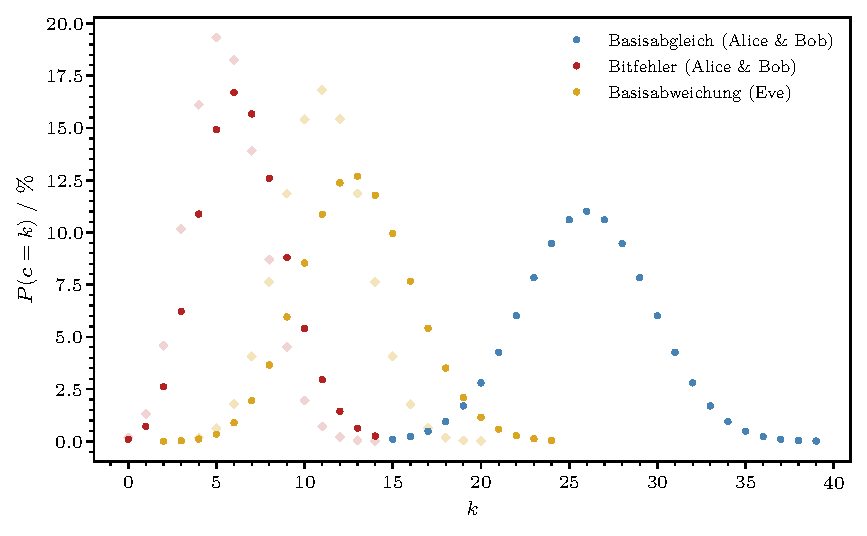
\includegraphics{build/verteilung.pdf}
	\vspace{-1.5\baselineskip}
	\captionsetup{width=0.93\textwidth}
	\caption{Verteilungen für den Basisabgleich mit $p = \qty{50}{\percent}$ sowie dabei auftretende Abweichungen der Abhörbasis
			 mit $p = \qty{25}{\percent}$ und des übertragenen Bits mit $p = \qty{12.5}{\percent}$ aus $n = 52$ Signalen. Dazu
			 zeigen transparente Punkte die Verteilungen mit der gemessenen Anzahl der gleichen Basen als Vorwissen.}
	\label{fig:verteilung}
	\vspace{-2.5\baselineskip}
\end{figure}

In Abbildung \ref{fig:verteilung} sind die Wahrscheinlichkeitsverteilungen der untersuchten Ereignisse visualisiert. Es ergibt sich
$\qty{6.01}{\percent}$ für die gemessenen 22 gleichen Basisstellungen. Aus 52 Signalen entsprechen 11 mit $\qty{10.86}{\percent}$
einem Fehler von \glqq{Eve}\grqq{} bei übereinstimmenden Basen von \glqq{Alice}\grqq{} und \glqq{Bob}\grqq{}. Für 4 Bitfehler gilt
$\qty{10.88}{\percent}$ als Wahrscheinlichkeit. Wird für die abweichende Lauscherbasis und das inkorrekte Bit stattdessen $n = 22$
aus der Anzahl gleicher Basen von \glqq{Alice}\grqq{} und \glqq{Bob}\grqq{} angesetzt, gelten $p = \qty{50}{\percent}$ für ersteren
und $p = \qty{25}{\percent}$ für letzteren Fall. Dann folgt $\qty{16.82}{\percent}$ für 11 Basisfehler und $\qty{16.11}{\percent}$
für 4 Bitfehler. Alle Anzahlen liegen im jeweiligen Bereich der maximalen Wahrscheinlichkeit und sind somit plausible Werte für eine
fehlerfreie Durchfühurng der Messreihen.
